% Created 2023-01-25 śro 10:48
% Intended LaTeX compiler: pdflatex
\documentclass[11pt]{article}
\usepackage[utf8]{inputenc}
\usepackage[T1]{fontenc}
\usepackage{graphicx}
\usepackage{longtable}
\usepackage{wrapfig}
\usepackage{rotating}
\usepackage[normalem]{ulem}
\usepackage{amsmath}
\usepackage{amssymb}
\usepackage{capt-of}
\usepackage{hyperref}
\makeatletter \@ifpackageloaded{geometry}{\geometry{ a4paper, total={170mm,257mm}, left=15mm, top=15mm }}{\usepackage[margin=1.5cm]{geometry}} \makeatother
\author{Dawid Jarosz, Tomasz Kolbusz}
\date{\today}
\title{Słupy oświetleniowe}
\hypersetup{
 pdfauthor={Dawid Jarosz, Tomasz Kolbusz},
 pdftitle={Słupy oświetleniowe},
 pdfkeywords={},
 pdfsubject={},
 pdfcreator={Emacs 28.2 (Org mode 9.5.5)}, 
 pdflang={English}}
\begin{document}

\maketitle
\tableofcontents


\section{Słupy oświetleniowe}
\label{sec:org0fc4196}

\subsection{Cel projektu}
\label{sec:org96f53b2}
Projekt ma za zadanie rozmieścić na mapie miasta słupy oświetleniowe co określoną odległość w pasie drogowym. Słupy nie mogą stać w tym samym miejscu co elementy infrastruktury miasta tj. bramy wjazdowe, chodniki.

\subsection{Dane wejściowe}
\label{sec:org076853f}

Jako zbiór danych używamy mapy drogowej oraz infrastruktury miasta Washington DC. Dane pochodzą z serwisu [\ldots{}tutaj link]. Wykorzystaliśmy dane dostępne w zbiorach Roads i Structure\textsubscript{Lines}. Zbiory pobraliśmy w formacie shp, pozwoli to na łatwe załadowanie ich do bazy danych.

\subsection{Wykorzystane technologie}
\label{sec:orge1bc8dc}

Do przechowywania danych i ich przetwarzania wykorzystujemy PostgreSQL wraz z rozszerzeniem PostGIS. Do skryptu wyznaczającego położenie słupów wykorzystujemy Deno.

\subsection{Podział prac}
\label{sec:orgd23b649}

Tomasz Kolbusz wymyślił wstępny algorytm, który w późniejszym etapie okazał się niewystarczający.

Dawid Jarosz ulepszył algorytm, który został wspólnie zaimplementowany.

\subsection{Uruchomienie aplikacji}
\label{sec:org00b981a}

\subsubsection{Załadowanie danych}
\label{sec:org1a3c12c}

Do załadowania danych z plików shp używamy programu shp2sql. Flaga -D zmienia format wyjściowy z programu na postgres'owy dump, przyspiesza to ładowanie danych. Flaga -I dokłada indeksy GiST na kolumny z geometrią.

\begin{verbatim}
shp2pgsql -D -I -s 4326 Structure_Lines_1999.shp Structure_Lines | psql 

shp2pgsql -D -I -s 4326 Roads.shp Roads | psql 
\end{verbatim}

\subsubsection{Uruchomienie skryptu}
\label{sec:org3893847}

Skrypt jest uruchamiany w deno, czyli środowisku uruchomieniowym typescript. Jedną z cech deno jest brak konieczności instalacji zależności. Zostaną one automatycznie pobrane przy starcie skryptu. Sam skrypt pozwala nam wywołać kolejne polecenia SQL za pomocą których wyznaczamy położenie słupów oświetleniowych.

\begin{verbatim}
deno run --allow-net app.ts 
\end{verbatim}

\subsection{Algorytm}
\label{sec:orge206f0d}

\begin{enumerate}
\item Wczytanie danych do bazy oraz utworzenie potrzebnych tabel.
\item Wczytanie ze zbioru Roads wszystkich obiektów według typów, wczytanie danych ze zbioru structure\textsubscript{lines}
\end{enumerate}

\begin{verbatim}
insert into objects2 select descriptio, st_transform(geom, 2855) from roads;

insert into structures2 select st_transform(geom, 2855) from structure_lines;
\end{verbatim}

\begin{center}
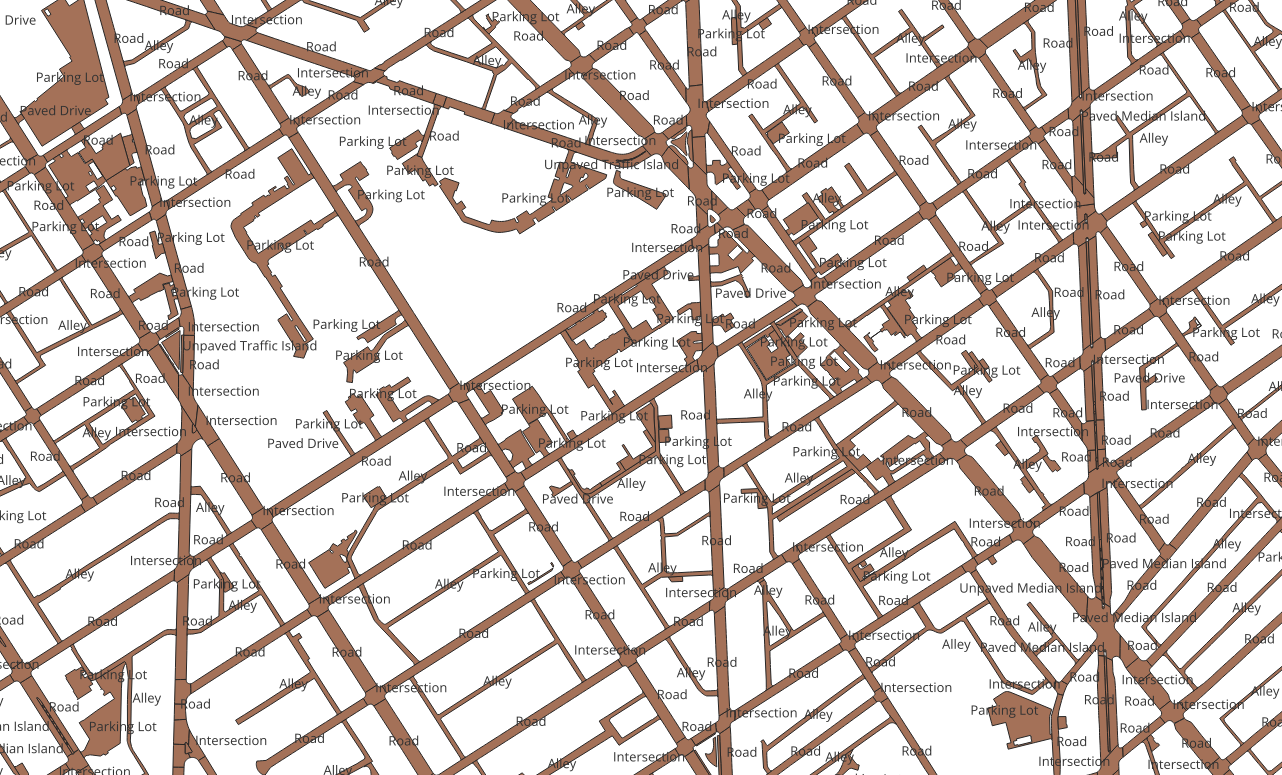
\includegraphics[width=.9\linewidth]{./img/1.png}
\end{center}

\begin{center}
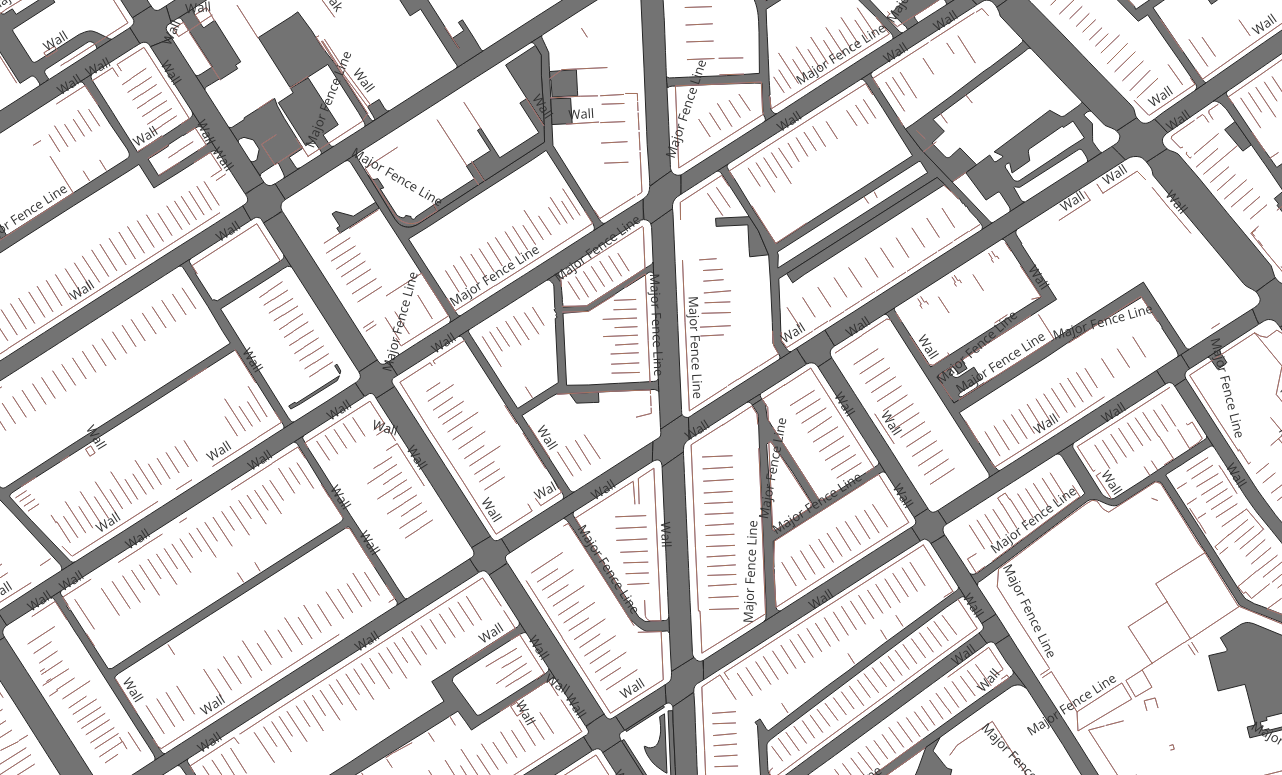
\includegraphics[width=.9\linewidth]{./img/10.png}
\end{center}

\begin{enumerate}
\item Wyciągnięcie konturów dróg
\end{enumerate}

Wykorzystując st\textsubscript{boundary} i st\textsubscript{buffer} możemy wytyczyć obrys drogi w zadanej odległości.

\begin{verbatim}
insert into roadsContours
select
    (st_dump(st_boundary(st_union(st_buffer(geom, ${distanceFromRoad}))))).geom
from objects
where description = 'Road' or description = 'Intersection';
\end{verbatim}

\begin{center}
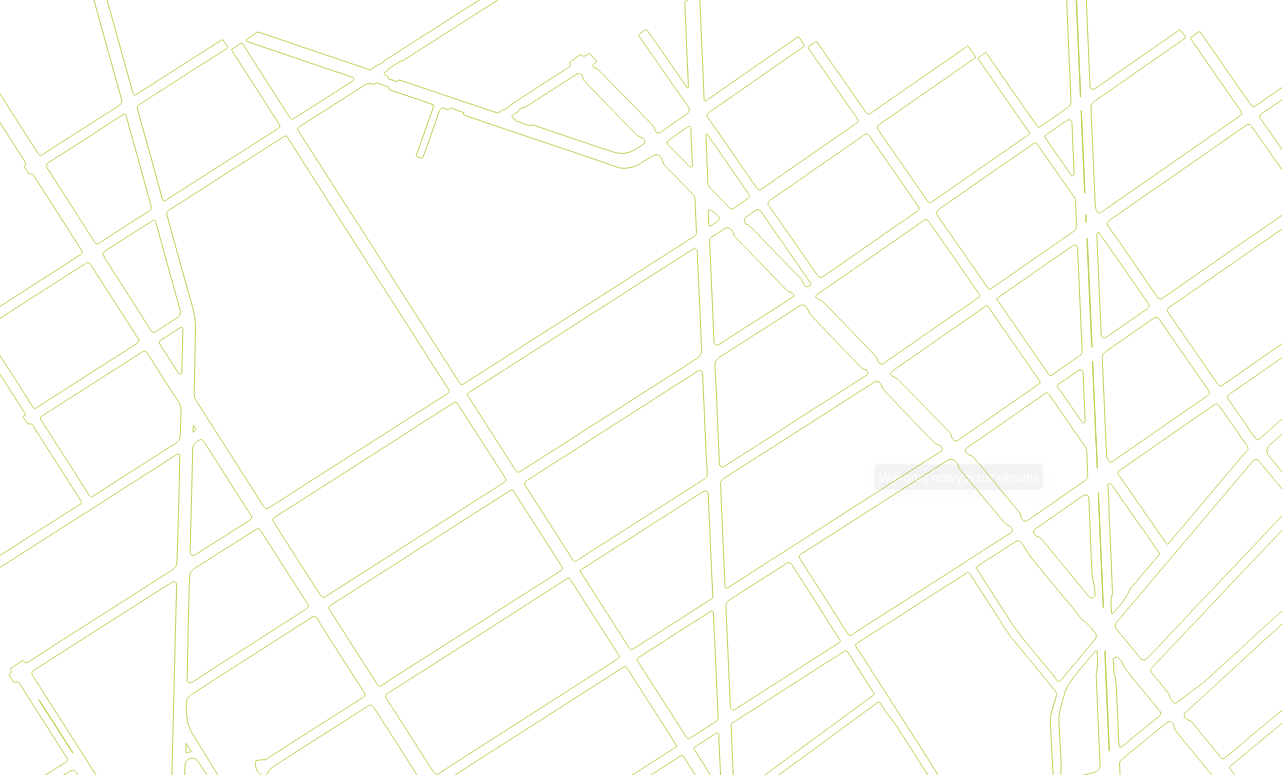
\includegraphics[width=.9\linewidth]{./img/2.png}
\end{center}



\begin{enumerate}
\item Ustawienie słupów wzdłuż dorgi co określony dystans
\end{enumerate}

Do wyznaczenia początkowego położenia słupów wykorzystujemy funkcje st\textsubscript{lineinterpolatepoints}, która pozwala wyznaczyć punkty na lini co zadany dystans. 

\begin{verbatim}
insert into initialPolesPlacement 
select st_lineinterpolatepoints(geom, ${poleSpacing}/st_length(geom)) 
from roadsContours 
where st_length(geom) > ${poleSpacing};
\end{verbatim}

\begin{center}
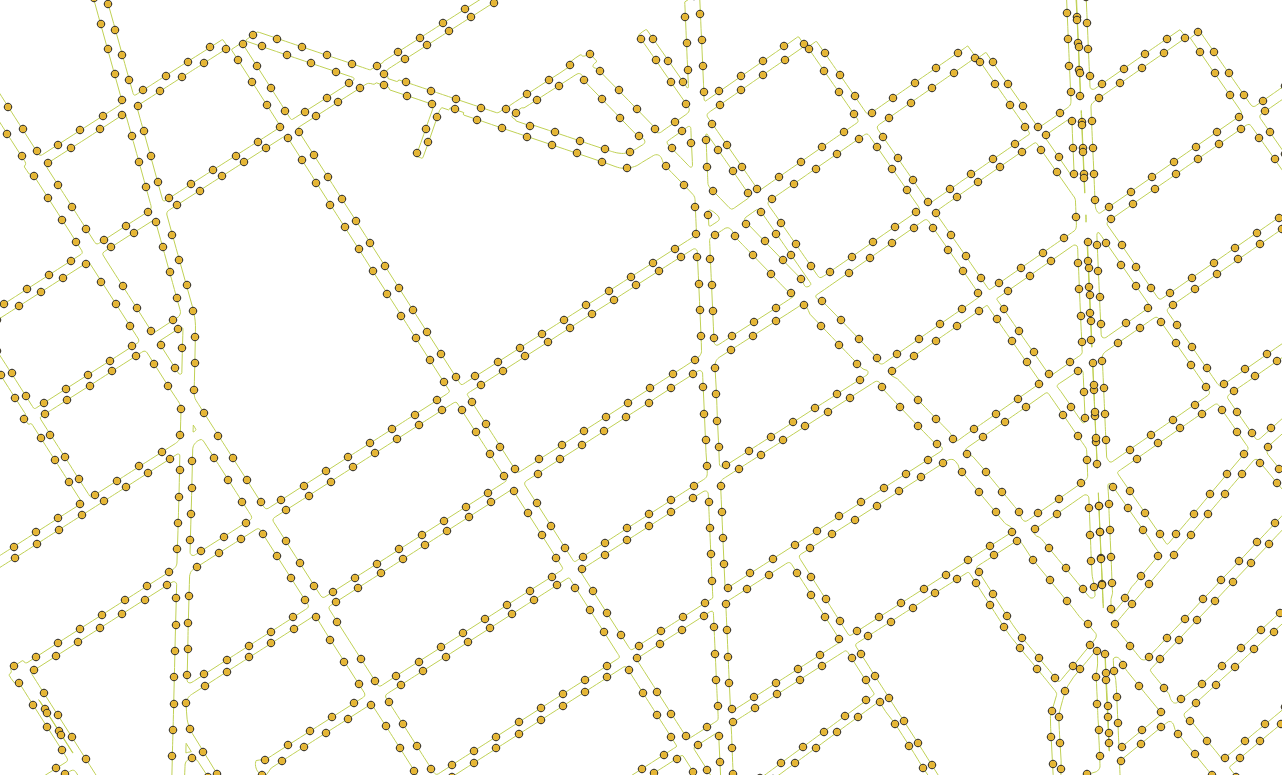
\includegraphics[width=.9\linewidth]{./img/3.png}
\end{center}

\begin{enumerate}
\item Rozwiązanie problemu skrzyżowań
\end{enumerate}

W przypadku skrzyżowań, nie chcieliśmy żeby nasz algorytm ustawił słupy w bliskiej odległości od skrzyżowania, a jednocześnie żeby w pewnej zadanej odległości ustawić słupy, które mogłyby doświetlać przejścia dla pieszych. 

a. Wyznaczenie dwóch stref wokoło skrzyżowania 

W tym punkcie wyznaczamy dwie strefy - większą z której usuniemy postawione słupy, drugą mniejszą, której przeciecie krawędzi z liniami według których wyznaczaliśmy pierwotne położenie słupów. Pozwoli to nam ustawić słupy w zadanej odległości od skrzyżowania (można wykorzystać jako oświetlenie przejść), a uniknąć sytuacji w której postawione słupy będą znajdować się bardzo blisko już postawionych słupów.

\begin{verbatim}
insert into intersections 
select 'clearZone', st_union(st_buffer(geom, ${clearZoneSize})) 
from objects 
where description = 'Intersection';

insert into intersections 
select 'placeZone', st_union(st_buffer(geom, ${placeZoneSize})) 
from objects 
where description = 'Intersection';
\end{verbatim}

\begin{center}
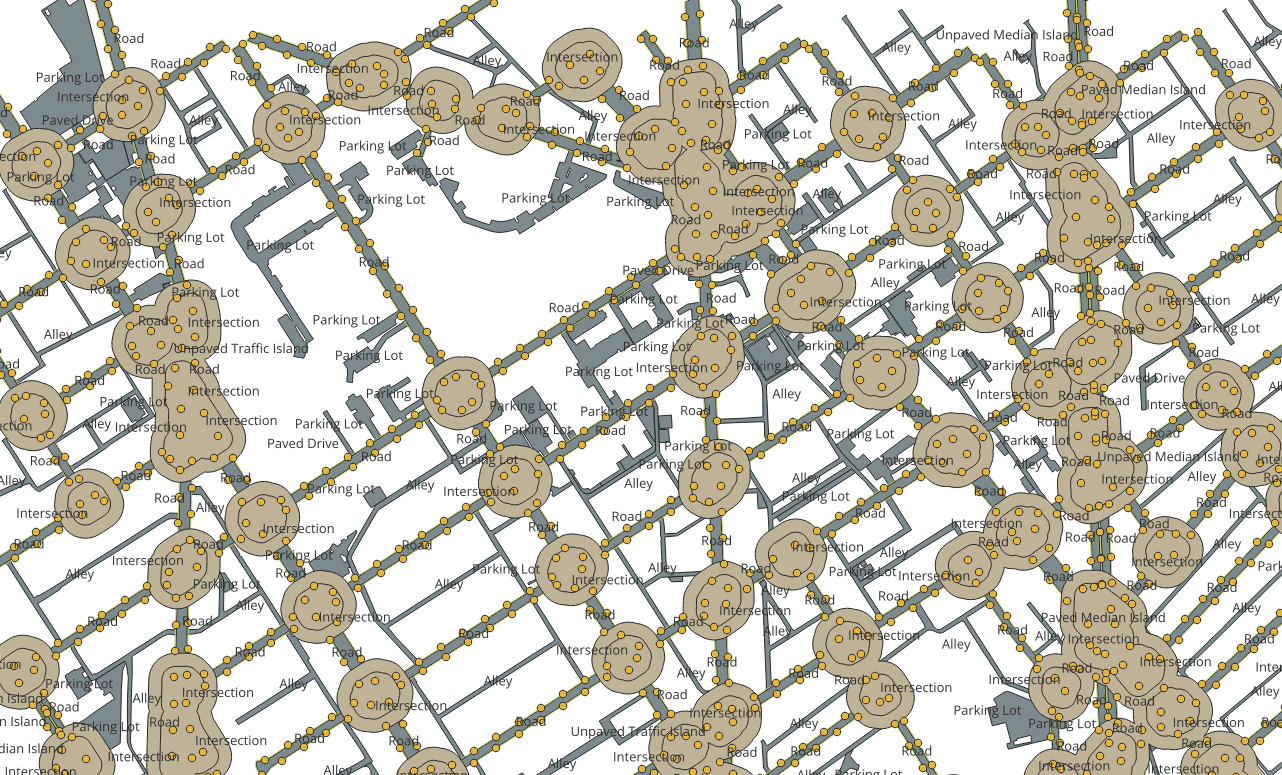
\includegraphics[width=.9\linewidth]{./img/4.png}
\end{center}

b. Usunięcie słupów z większej strefy

\begin{verbatim}
insert into polesAfterIntersections 
select (st_dump(st_difference(
    (select st_union(geom) from initialpolesplacement), 
    (select st_union(geom) from intersections where type = 'clearZone')))
).geom;
\end{verbatim}

c. Dodanie słupów na przecięciach 

\begin{verbatim}
insert into polesAfterIntersections 
select st_intersection(
    (select st_boundary(st_union(geom)) from intersections where type = 'placeZone'), 
    (select st_union(geom) from roadsContours)
);
\end{verbatim}

\begin{center}
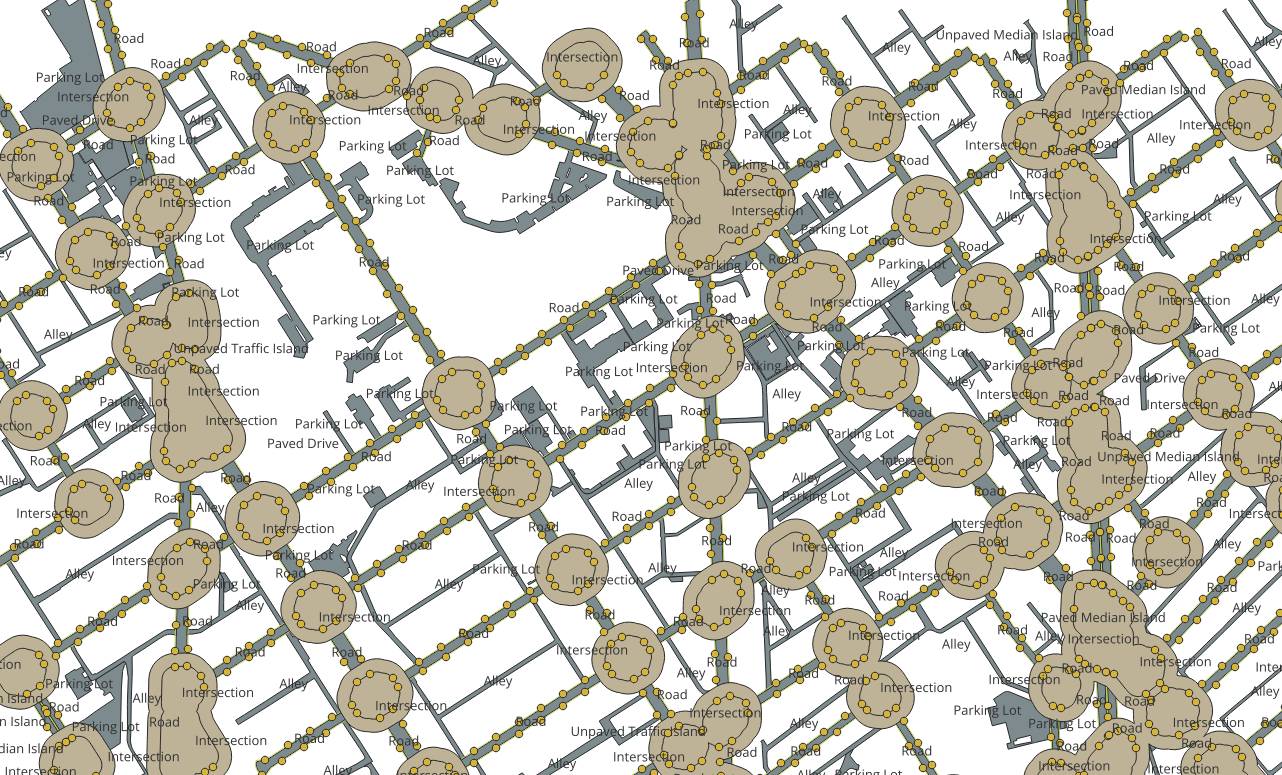
\includegraphics[width=.9\linewidth]{./img/5.png}
\end{center}

\begin{enumerate}
\item Znalezienie przeszkód które uniemożliwiają postawienie słupów.
\end{enumerate}

Tutaj jako przeszkody zakwalifikowaliśmy pozostałe obiekty ze zbioru Roads, takie jak alejki, parkingi, podjazdy oraz zbiór Structure\textsubscript{Lines}.

\begin{verbatim}
insert into obstacles 
select st_buffer(st_union(geom), 3) 
from objects 
where description != 'Road' and description != 'Intersection';
\end{verbatim}

\begin{center}
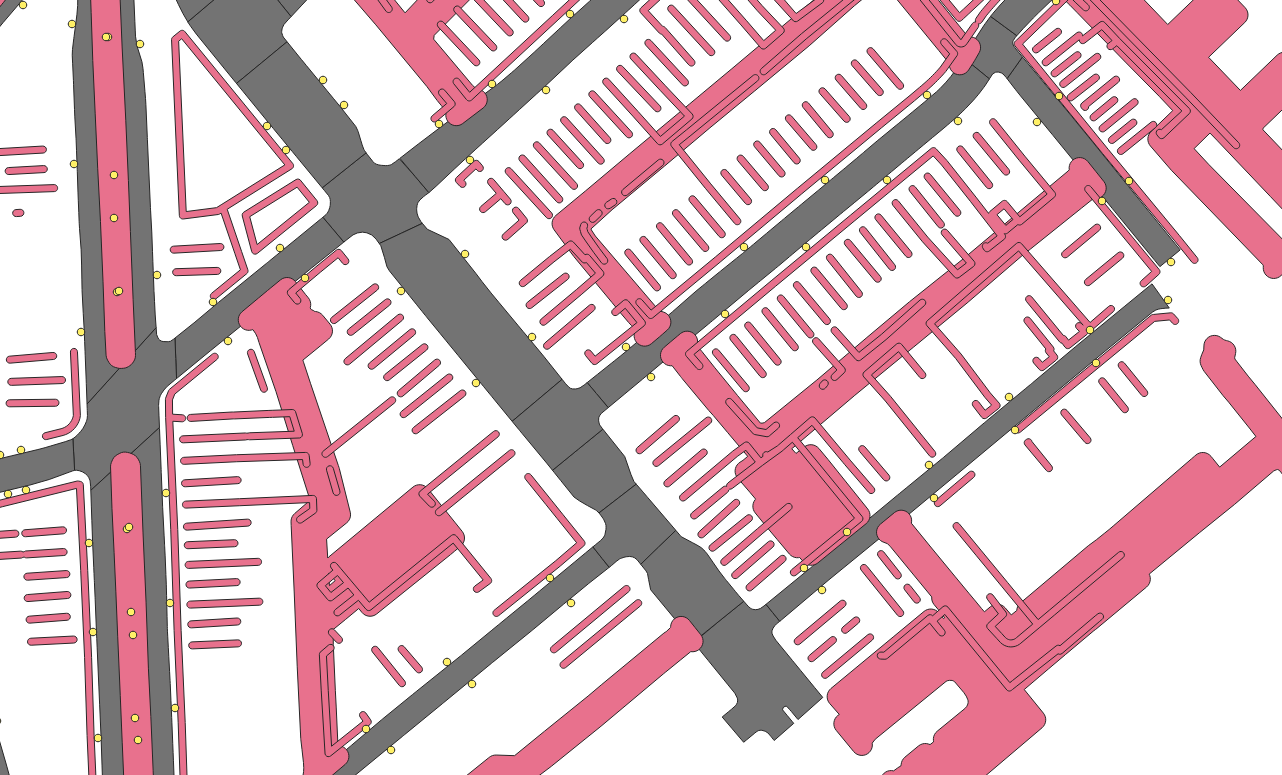
\includegraphics[width=.9\linewidth]{./img/6.png}
\end{center}

\begin{enumerate}
\item Usunięcie słupów które kolidują z przeszkodami.
\end{enumerate}

\begin{verbatim}
insert into clearedFromObstacles 
select (st_dump(st_difference(
    (select st_union(geom) from polesAfterIntersections),
    (select st_union(geom) from obstacles)))
).geom;
\end{verbatim}

\begin{enumerate}
\item Rozwiązanie problemu z brakującymi słupami po usunięciu kolidujących.
\end{enumerate}

Po usunięciu kolidujących słupów odległości między niektórymi słupami mogą być znacznie większe niż założone, dlatego postanowiliśmy usunięte punkty przesunąć na pozycję na której nie będą kolidowały z innymi obiektami. 

a. Wybranie uniętych punktów.

\begin{verbatim}
insert into toMove 
select (st_dump(st_intersection(
    (select st_union(geom) from polesAfterIntersections), 
    (select st_union(geom) from obstacles)))
).geom;
\end{verbatim}

b. Znalezienie lini według których były ustawiane słupy, ale wycięcie części które kolidują z obiektami

\begin{verbatim}
insert into contoursWithoutObstacles 
select st_difference(
    (select st_union(geom) from roadscontours), 
    (select st_union(geom) from obstacles)
);
\end{verbatim}

c. Znalezienie najbliższych punktów, które nie kolidują z przeszkodami. 

W tym miejscu dla każdego usuniętego punktu szukamy najbliższego możliwego położenia dla punktu. Efektywnie to przesuwa punkt na lini która przechodzi przez tą przeszkodę, stawiając go po najbliższej stronie przeszkody.

\begin{verbatim}
insert into movedPoints 
select st_closestPoint((select geom from contoursWithoutObstacles), geom) 
from tomove;
\end{verbatim}

\begin{center}
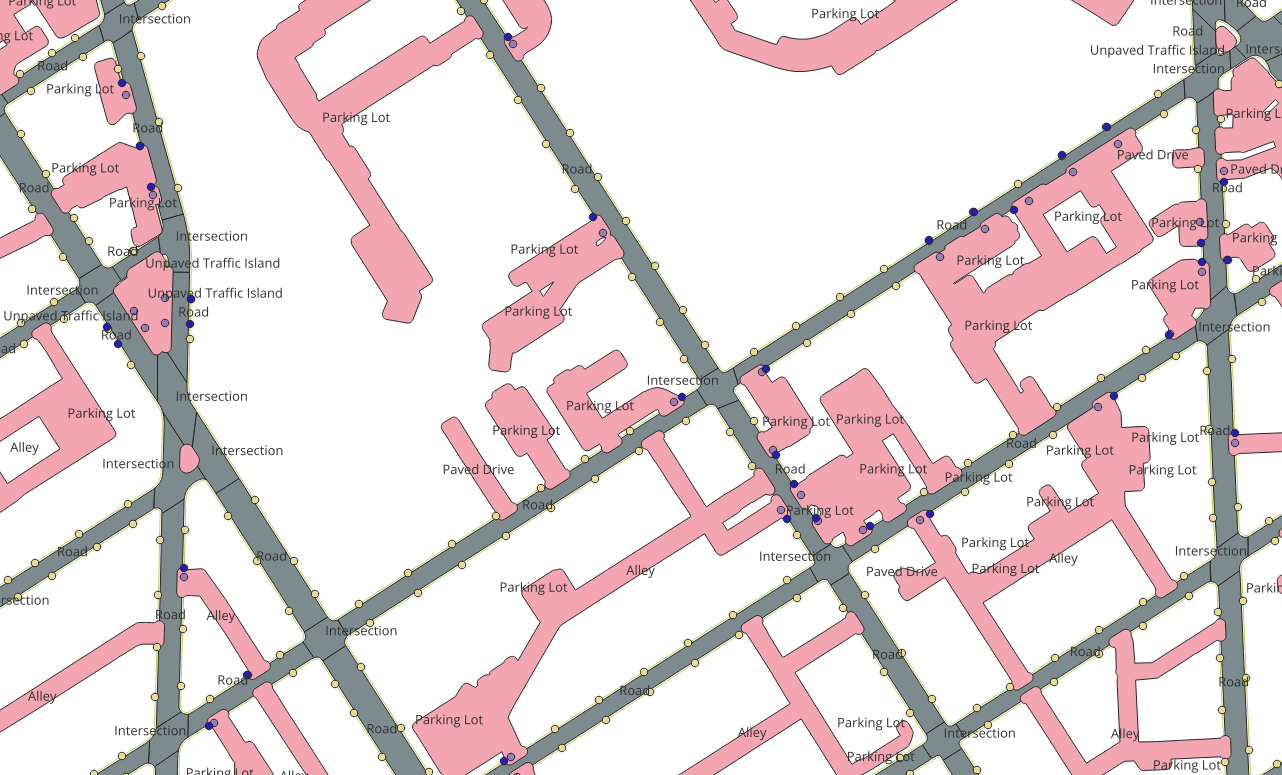
\includegraphics[width=.9\linewidth]{./img/7.png}
\end{center}

Fioletowe punkty zostały przesunięte do pozycji niebieskich punktów.

\begin{enumerate}
\item Znalezienie punktów które postawione są za blisko siebie i usunięcie ich.

\begin{verbatim}
insert into finalPoles select ST_RemoveRepeatedPoints(st_collect(geom), ${minLength}) from clearedFromObstacles;
\end{verbatim}
\end{enumerate}

\begin{center}
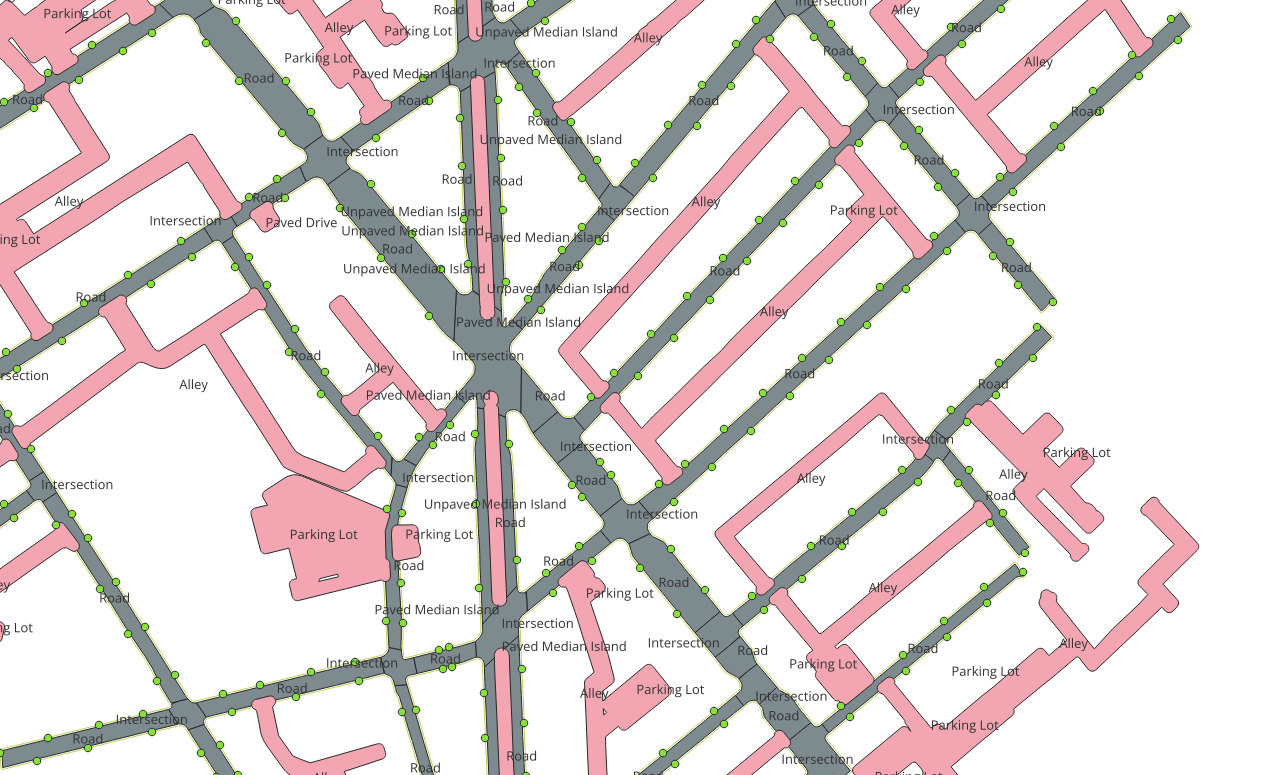
\includegraphics[width=.9\linewidth]{./img/8.png}
\end{center}

\begin{center}
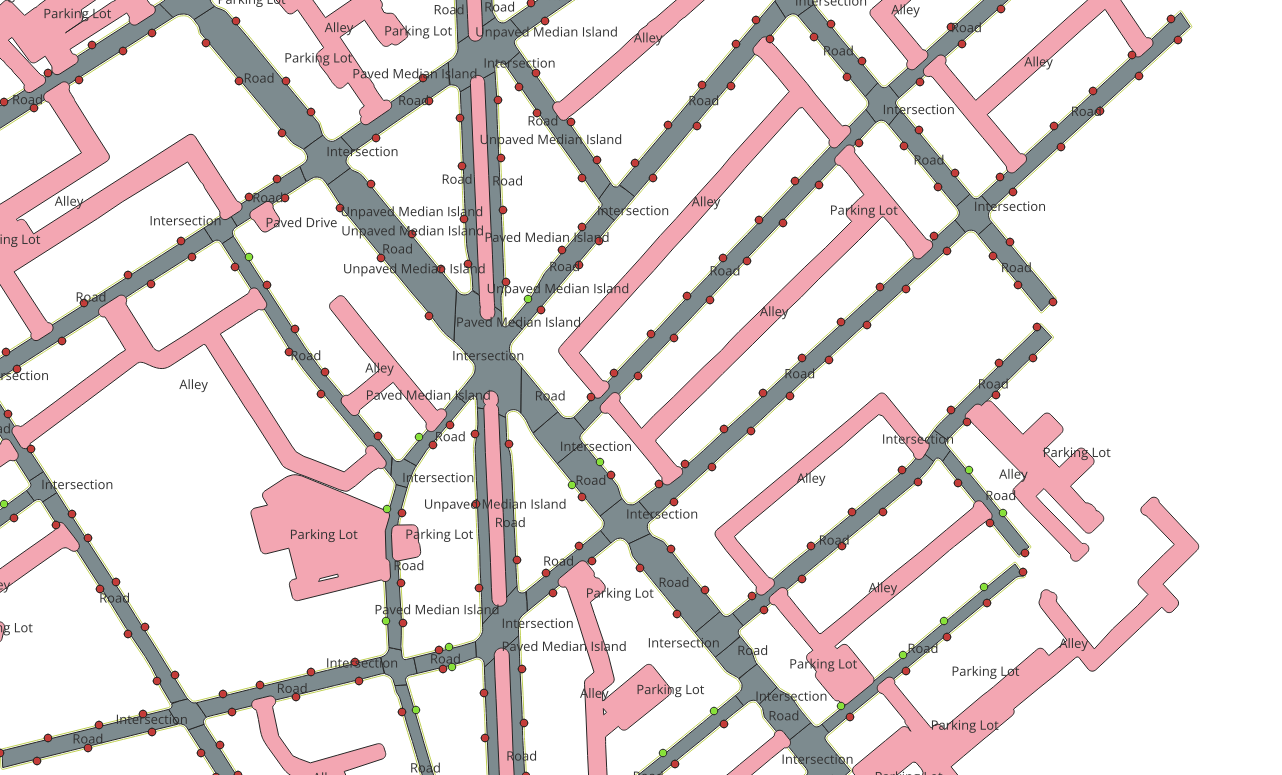
\includegraphics[width=.9\linewidth]{./img/9.png}
\end{center}
\end{document}